\documentclass[lectures, draft]{pcms-l}


% Preamble

% Please put all macro definitions and package calls in this preamble
% area. 

\usepackage{verbatim}
\usepackage{graphicx}

\theoremstyle{plain}
\newtheorem{theorem}{Theorem}[chapter]
\newtheorem{lemma}{Lemma}[chapter]
\newtheorem{proposition}{Proposition}[chapter]
\newtheorem{corollary}{Corollary}[chapter]

\theoremstyle{definition}
\newtheorem{definition}{Definition}[chapter]
\newtheorem{example}{Example}[chapter]
\newtheorem{exercise}{Exercise}[lecture]

\theoremstyle{remark}
\newtheorem{remark}{Remark}[lecture]

% To properly number equations, edit and uncomment  

\numberwithin{equation}{chapter}


\newcommand\pcms{\texttt{pcms-l.cls}}
\newcommand\amsbook{\texttt{amsbook.cls}}

% \renewcommand\thesection{\thechapter.\arabic{section}}
% \renewcommand\thesubsection{\thesection.\arabic{subsection}}
% \renewcommand\thesubsubsection{\thesubsection.\arabic{subsubsection}}

\begin{document}

\frontmatter
\tableofcontents

\mainmatter

\LectureSeries[PCMI Lecture Notes]%
{Preparation of PCMI~Lecture~Notes \author{John C. Polking}}


\address{Department of Mathematics, MS 136, Rice University, PO Box
  1892, Houston, TX 77251} 

\email{polking@rice.edu}

\thanks{I would like to thank Barbara Beeton of the American
  Mathematical Society for writing pcms-l.cls, the \TeX\ document class in
  which these notes were typed.}


\section*{Introduction}
These notes are provided in order to simplify and uniformize the
preparation of the lectures notes for the Graduate Summer School at
the Park City Mathematical Institute.  

Since the notes for the various lecture series eventually appear in
one volume, we want to ensure some uniformity of appearance.  At the
same time we want to make the preparation of the notes as easy as
possible for the lecturers.  To this end the American Mathematical
Society (AMS) provides us with a document class file, \pcms.  This is
based on the AMS book document class, \amsbook.

This document is (rather artificially) prepared using \pcms\ in order
to provide a sample of its use.  The niceties of this document class
are explained in the first lecture.

The second lecture is devoted to the use of \AmS-\LaTeX\ to typeset
mathematics.  Specific examples are presented so that this document
can serve as a robust model of a PCMI lecture series.

In the third lecture we discuss the use of graphics in the lecture
notes.  In particular we explain the limits that the AMS puts on the
use of graphics.  We also offer some advice on how to meet those
limits.

The fourth lecture contains a list of resources for the use of \TeX\
and \AmS-\LaTeX.

\lecture{The PCMI Document Class}

The class \pcms\ is a \LaTeXe\ document class developed by the AMS\@.
It modifies \amsbook\ to allow the use of the lecture format seen in
this document.  The lecture format is the preferred format for the
PCMI lectures.  However, if he or she prefers, a lecturer may present
the material of the lecture series in an article format.  Both formats
are described here.

In order to use \pcms\ you will need a \TeX\ installation on your
computer and the class file \amsbook\ installed.  The AMS \TeX\ 
Resources Home Page (http://www.ams.org/tex/) is a starting point for
both.  It provides links to sources for \TeX\ and \LaTeX\ as well to
sources of information about setting up a \TeX\ installation.  It also
provides a link to the \AmS-\LaTeX\ collection.  If your \LaTeX\ 
installation is recent (after August 2004), you should already have
\amsbook\ installed.  If not, you should download and install the
entire \AmS-\LaTeX\ collection.


\section{The organization of a file in the lecture format.}

Your lecture \TeX\ file should follow the standard outline of a
\LaTeXe\ file.  We will describe that organization in what follows.
You can find more detail in \cite{gratz} or \cite{guide}.

\subsection{The document class declaration}

The document should start with the document class declaration
\begin{verbatim}
\documentclass[lectures]{pcms-l}
\end{verbatim}
The option \verb-lectures- indicates that this file will use the
lecture format.  The alternative would be \verb-article-.

You can also add other \LaTeXe\ options.  In particular you might use
the \verb-draft- option to clearly mark the overfull lines which you
will want to eliminate before submitting your manuscript.  To do this
use the declaration 
\begin{verbatim}
\documentclass[lectures, draft]{pcms-l}
\end{verbatim}

\subsection{The preamble}
This is the place to input the extra packages that you use, to set up
your declarations for theorems, lemmas, definitions, etc., and to 
define your own macros.
\subsubsection{Packages}  Since \pcms\ is based on \amsbook, which
automatically loads the \verb-amsmath- and \verb-amsfonts- packages,
it is not necessary to input these.  However, you will undoubtedly use
others.  In particular, if you have any graphics, you will want to use
the \verb-graphicx- package.  Thus you will have a section that
resembles 
\begin{verbatim}
\usepackage{graphicx}
\usepackage{amssymb}
\usepackage{mathrsfs}
\usepackage{latexsym}
\usepackage{verbatim}
\end{verbatim}

Please list only those packages you actually use.

\subsubsection{Theorem-like declarations} \label{theorems} One of the
nicer features of \LaTeXe\ is the ease with which these declarations
can be made.  Thus you might include a list something like
\begin{verbatim}
\theoremstyle{plain}
\newtheorem{thm}{Theorem}
\newtheorem{lem}{Lemma}
\newtheorem{prop}{Proposition}
\newtheorem{cor}{Corollary}

\theoremstyle{definition}
\newtheorem{def}{Definition}
\newtheorem{example}{Example}
\newtheorem{exer}{Exercise}

\theoremstyle{remark}
\newtheorem{rem}{Remark}
\end{verbatim}
\enlargethispage{10pt}

There are three different ``theorem'' styles available:
\begin{itemize}
\item {\texttt{plain}} -- the text is in the italic font with extra
  space above and below.
\item {\texttt{definition}} -- the text is in the roman font with extra
  space above and below.
\item {\texttt{remark}} -- the text is in the roman font with no extra
  space above and below.
\end{itemize}

You can find more information about theorem-like declarations in
\cite{amsmath}, \cite{amsthm}, \cite{gratz}, and \cite{guide}.

\subsubsection{Numbering}  \label{numbs}The above theorem-like
declarations will result in each of the items being numbered
separately in one string throughout the manuscript.  More than likely
this is not what you want.  Many people think it is more natural to
restart the numbering in each lecture and precede the number with the
lecture number.  This can be achieved by adding a counter option to
each declaration.  For example,
\begin{verbatim}
\newtheorem{lem}{Lemma}[chapter]
\end{verbatim}
will do the job for your lemmas.  (This is currently a bug in \pcms.
The option should really be \verb-[lecture]-, but \verb-[chapter]- is
what works.)

To number equations by lecture use the command
\begin{verbatim}
\numberwithin{equation}{chapter}
\end{verbatim}
(Again we have the bug.)

Some people like to number theorems, lemmas, propositions,
corollaries, and perhaps other things together in one series.  This
can be accomplished with the commands
\begin{verbatim}
\newtheorem{theorem}{Theorem}[chapter]
\newtheorem{lemma}[theorem]{Lemma}
\newtheorem{proposition}[theorem]{Proposition}
\newtheorem{corollary}[theorem]{Corollary}
\end{verbatim}
It is essential that the Theorem declaration appear first in this list
of commands. 

\subsubsection{Macros}  Everyone has their own macros.   These should
all be included in the preamble.  The primary reason for this is that
it makes things a whole lot easier for editors. Have pity on us.  

For example, in this document we use the macros
\begin{verbatim}
\newcommand\pcms{\texttt{pcms-l.cls}}
\newcommand\amsbook{\texttt{amsbook.cls}}
\end{verbatim}

\subsection{Preparation for the  main part of the document}
After the preamble we are almost ready for the mathematics.  Some
preparation is required, however.  As an example, the main part of
this document starts with the commands
\begin{verbatim}
\begin{document}

\frontmatter
% \tableofcontents

\mainmatter

\LectureSeries[PCMI Lecture Notes]%
{Preparation of PCMI Lecture Notes \author{John C. Polking}}

\address{Department of Mathematics, MS 136, Rice University, PO Box
  1892, Houston, TX 77251} 

\email{polking@rice.edu}

\section*{Introduction}

\end{verbatim}
\subsubsection{Document environment}
Everything from this point on is done in the document environment. That
means that everything is placed between the two commands
\begin{verbatim}
\begin{document}
...
\end{document}
\end{verbatim}
 The command
\verb-\end{document}- should be the last line in the file.
\subsubsection{The front matter}
This simply amounts to 
\begin{verbatim}
\frontmatter
\tableofcontents
\end{verbatim}
The command \verb-\tableofcontents- will cause a table of contents to
be developed.  That is not essential until the final document is
assembled, but you might like to see it anyway.
\subsubsection{Main matter}
This starts with two commands
\begin{verbatim}
\mainmatter
\LectureSeries[short-name]{long-name \author{author-name}}
\end{verbatim}
In \verb-\LectureSeries-, \verb=short-name= is a shortened name for
the lecture series suitable for appearance in page headers, while
\verb=long-name= is the real name for the series.  
Notice how \verb=\author{author-name}= appears within the curly brackets for
\verb=long-name=. 

Next we need some information about the author.  The commands 
\begin{verbatim}
\address{author-address} 
\email{author-email-address}
%%\subjclass[2000]{Primary}
%% \keywords{}
%% \date{}
%% \thanks{}
\end{verbatim}
should be self-explanatory.  The items that are commented out are
optional.  However, please provide your official mailing and email
adresses.  


\subsection{Introductory material}
Almost every lecture series begins an introductory section with a
title like ``Introduction'', or ``Preface'', or perhaps something more
inventive.  Start such a section with the command
\begin{verbatim}
\section*{intro-name}
\end{verbatim}
The asterisk will ensure that the section is not numbered.  There can
be two or more such sections. 

\subsection{Subdivisions of the document}
Each lecture is originated with the command
\begin{verbatim}
\lecture{lecture-name}
\end{verbatim}
In the compiled document each new lecture starts on a new odd-numbered
page.

Within a lecture the author has available sections, subsections, and
subsubsections.  These are called with the commands
\begin{verbatim}
\section{section-name}
\subsection{subsection-name}
\subsubsection{subsubsection-name}
\end{verbatim}
The effect of these commands is illustrated in this document. 

\subsection{The bibliography}
This is prepared in the way that is standard in \LaTeXe, and is explained
in \cite{guide}.  


\section{The organization of a file in article format}
The article format is essentially one lecture without a beginning
\verb-\lecture- command.  There are only three differences about
preparing a manuscript in the article format.  We will only describe
these few differences.

First of all, the document class declaration should be 
\begin{verbatim}
\documentclass[article]{pcms-l}
\end{verbatim}

The second difference is that the only subdivisions that are available
are the section, subsection, and subsubsection.  There is no lecture
division.  The major subdivisions of the manuscript are sections.  The
sections should be started with the command
\begin{verbatim}
\section[short section name]{section name}
\end{verbatim}
The short section name is needed only if the section name is too long to
fit in the header of the even numbered pages.
%\enlargethispage{10pt}

Finally, since there is no lecture division, we cannot number
equations, theorems, etc., by lecture.  A suitable modification is to
do so by section.  This requires that the theorem-like declarations
should read
\begin{verbatim}
\newtheorem{theorem}{Theorem}[section]
\end{verbatim}
Notice that we are using the counter \verb-section- instead of
\verb-chapter- as we did in~\ref{numbs}.  It will also be necessary to
add the command
\begin{verbatim}
\numberwithin{equation}{section}
\end{verbatim}
so that the equations are numbered by section. 

\lecture{\AmS-\LaTeX\ Examples}

Here we will summarize the most important methods for putting
mathematical formulas into a \TeX\ document.  At the risk of boring
the experienced reader we will start with the easiest examples.
\section{Math within text}
The original way of doing this in \TeX\ is to use the dollar sign
symbol. 
\begin{verbatim}
The commutative law says that $x+y = y+x$.
\end{verbatim}
\LaTeX\ provides two other ways,
\begin{verbatim}
The commutative law says that \(x+y = y+x\).
\end{verbatim}
and
\begin{verbatim}
The commutative law says that \begin{math}x+y = y+x\end{math}.
\end{verbatim}

Any of these three will produce

\medskip
The commutative law says that \begin{math}x+y = y+x\end{math}.
\medskip

\noindent
Most people think that the use of \verb-$x+y = y+x$- is still the most
convenient. 

\section{Single line displayed formulas}
\subsection{Unnumbered equations}
The original \TeX\ way is to use the double dollar sign
\begin{verbatim}
$$x+y=y+x$$
\end{verbatim}
\LaTeX\ again provides two other  ways
\begin{verbatim}
\begin{displaymath}
  x+y=y+x
\end{displaymath}
\end{verbatim}
and
\begin{verbatim}
\[x+y=y+x\]
\end{verbatim}
In addition, \AmS-\LaTeX\ allows the use of the starred
\texttt{equation} environment
\begin{verbatim}
\begin{equation*}
  x+y=y+x
\end{equation*}
\end{verbatim}
Any of these four ways will produce the display
\[x+y=y+x.\]

\subsection{Numbered equations}
To add a reference number to an equation, use the unstarred
\texttt{equation} environment
\begin{verbatim}
\begin{equation}
  \label{commlaw}
  x+y=y+x
\end{equation}
\end{verbatim}
This will produce 
\begin{equation}
  \label{commlaw}
  x+y=y+x
\end{equation}
The command \verb-\label{commlaw}- allows us to easily refer back to
the commutative law~\eqref{commlaw} with the command
\verb-\eqref{commlaw}-.  Notice that we used \verb-\eqref- and not
\verb-\ref-.  The later command would provide the equation number
without the parentheses. 

\section{Multiline displays}
For this purpose \LaTeX\ provides the \verb-eqnarray- environment.
This environment produces very bad spacing, and it is not recommended.
To replace it, the \AmS-\LaTeX\ package adds the following six
environments:
\begin{verbatim}
         align   gather   falign   multiline  alignat  split
\end{verbatim}
With the exception of the \texttt{split} environment, each has both
a starred and an unstarred form.  

Clearly, there are a lot of options.  So many that it is difficult to
learn them all.  However, I suggest that almost everything can be done
quite easily using only the \texttt{align} and \texttt{split}
environments in their starred and unstarred forms.  This is
demonstrated in the examples that follow.

\subsection{Aligned equations with all equations numbered}
This is produced by the unstarred \texttt{align} environment.  For
example
\begin{verbatim}
\begin{align}
  x + y &= y + x,\label{addcomm}\\
  xy &= yx.\label{multcomm}
\end{align}
\end{verbatim}
produces
\begin{align}
  x+y&=y+x,\label{addcomm}\\
  xy&=yx.\label{multcomm}
\end{align}

Notice that \verb-\\- is the end of line command, and that the
ampersand \verb-&- is the alignment character, which tells \TeX\ where
to match up the two lines.  In order to get correct spacing, the
alignment character should always be placed directly before the
character you want to align on.  Thus, you should use \verb-&=- and
not \verb-& =-.


Again, we can refer to the commutative law
for multiplication \eqref{multcomm} with the command
\verb-\eqref{multcomm}-.

\subsection{Aligned equations with no equations numbered}
This is produced by the starred \texttt{align*} environment.  For
example
\begin{verbatim}
\begin{align*}
  x + y &= y + x,\\
  xy &= yx.
\end{align*}
\end{verbatim}
produces
\begin{align*}
  x+y&=y+x,\\
  xy&=yx.
\end{align*}

Thus the starred version \texttt{align*} omits the numbers, while the
unstarred version \texttt{align} assigns a number to every line.

\subsection{Displays with only some lines numbered}
The way to achieve this is to use the  \verb-\notag-
command.  For example,
\begin{verbatim}
\begin{align}
    x+y&=y+x,\label{addcomm3}\\
    xy&=yx.\notag
\end{align}
\end{verbatim}
produces
\begin{align}
    x+y&=y+x,\label{addcomm3}\\
    xy&=yx.\notag
\end{align}

\subsection{Equations too long for one line}
The \texttt{split} environment was invented to handle these
situations.  It provides a convenient way to split such an equation
into two or more lines with a single equation number nicely
positioned.  For example,
\begin{verbatim}
\begin{align}
  \begin{split}
    u(x,y) &= \sum_{n=1}^\infty a_n\sinh\left(\frac{n\pi y}a\right)
    \sin \left(\frac{n\pi x}a \right)\\
    &\quad +\sum_{n=1}^\infty b_n\sinh\left(\frac{n\pi(y-b)}a\right) 
    \sin \left(\frac{n\pi x}a \right)
  \end{split}\label{solsimplap}
\end{align}
\end{verbatim}
produces
\begin{align}
  \begin{split}
    u(x,y) &= \sum_{n=1}^\infty a_n\sinh\left(\frac{n\pi y}a\right)
    \sin
    \left(\frac{n\pi x}a \right)\\
    & \quad + \sum_{n=1}^\infty b_n \sinh\left(\frac{n\pi
        (y-b)}a\right) \sin \left(\frac{n\pi x}a \right)
  \end{split}\label{solsimplap}
\end{align}
Notice that the equation number is centered so that it clearly refers
to both lines used to define $u$.


\subsection{Aligned equations with one number for all}
While \texttt{split} was invented to deal with splitting very long
equations, it can also be used effectively to group equations.  For
example, 
\begin{verbatim}
\begin{align}
  \begin{split}
    x+y&=y+x,\\
    xy&=yx.
  \end{split}  \label{commlaws}
\end{align}
\end{verbatim}
produces
\begin{align}
  \label{commlaws}
  \begin{split}
    x+y&=y+x,\\
    xy&=yx.
  \end{split}
\end{align}
Notice that there is one equation number, nicely centered between the
two lines.  We can refer to the commutative laws, \eqref{commlaws}, with the
command \verb-\eqref{commlaws}-.


\subsection{More complicated alignments}
Suppose we want to list the commutative laws followed by the
associative laws and then the distributive law, with one number for
each.  This can be done with
\begin{verbatim}
\begin{align}
  \begin{split}
    x+y&=y+x,\\
    xy&=yx,
  \end{split}\label{commlaws2}\\
  \begin{split}
    (x+y)+z & = x+(y+z),\\
    (xy)z &= x(yz),
  \end{split}\label{assoclaws}\\
  x(y+z) &= xy + xz.\label{distlaw}
\end{align}
\end{verbatim}
We get
\begin{align}
  \begin{split}
    x+y&=y+x,\\
    xy&=yx,
  \end{split}\label{commlaws2}\\
  \begin{split}
    (x+y)+z & = x+(y+z),\\
    (xy)z &= x(yz),
  \end{split}\label{assoclaws}\\
  x(y+z) &= xy + xz.\label{distlaw}
\end{align}
Notice that \TeX\ maintains the alignment even outside of each
\texttt{split} environment.

\subsection{Formulas in two or more columns}
The \texttt{align} environment allows the use of more than one
alignment character (\verb-&-).  This enables us to display formulas
in more than one column.  For example,
\begin{verbatim}
\begin{align}
  x + y   &= y + x,   &    xy &= yx,\label{commlaws3}\\
  (x+y)+z &= x+(y+z), & (xy)z &= x(yz).\label{assoclaws2}
\end{align}
\end{verbatim}
produces
\begin{align}
  x+y&=y+x, & xy&=yx,\label{commlaws3}\\
  (x+y)+z & = x+(y+z), & (xy)z &= x(yz).\label{assoclaws2}
\end{align}
Notice the different functionality of the odd-numbered and
even-numbered ampersands.  The odd-numbered ampersands are alignment
characters, while the even-numbered ones are column separators.  

\section{Theorem, lemmas, corollaries, definitions, etc.}
Having defined our theorem-like macros in the preamble, it is now easy
to use them.  For example,
\begin{verbatim}
\begin{definition}\label{compact}
  A set $K$ is compact if every open cover of $K$ has a 
  finite subcover.
\end{definition}
\end{verbatim}
produces
\begin{definition}\label{compact}
  A set $K$ is compact if every open cover of $K$ has a finite subcover.
\end{definition}

If you want to add a name to a definition you can do so in square
brackets.  Thus 
\begin{verbatim}
\begin{definition}[Compact set]\label{compact2}
  A set $K$ is compact if every open cover of $K$ has a 
  finite subcover.
\end{definition}
\end{verbatim}
produces
\begin{definition}[Compact set]\label{compact2}
  A set $K$ is compact if every open cover of $K$ has a finite subcover.
\end{definition}

The label allows us to refer to Definition~\ref{compact} as
\verb-Definition~\ref{compact}.- (The tilde (\verb-~-) is used to
prevent a line break between Definition and \ref{compact}.  It is not
needed here, but it is good to be sure.)

Theorems, etc., are handled similary.  Here are some examples. 

\begin{verbatim}
\begin{theorem}[Existence of solutions]\label{exist} 
  Suppose the function $f(t,x)$ is defined and continuous on the
  rectangle $R$ in the $tx$-plane. Then given any point
  $(t_0,x_0)\in R$, the initial value problem
  $$x' = f(t,x)\quad\text{and}\quad x(t_0) = x_0$$
  has a solution
  $x(t)$ defined in an interval containing $t_0$.  Furthermore, the
  solution will be defined at least until the solution curve
  $t\to(t,x(t))$ leaves the rectangle $R$.
\end{theorem}
\end{verbatim}
produces
\begin{theorem}[Existence of solutions]\label{exist} 
  Suppose the function $f(t,x)$ is defined and continuous on the
  rectangle $R$ in the $tx$-plane. Then given any point
  $(t_0,x_0)\in R$, the initial value problem
  $$x' = f(t,x)\quad\text{and}\quad x(t_0) = x_0$$
  has a solution
  $x(t)$ defined in an interval containing $t_0$.  Furthermore, the
  solution will be defined at least until the solution curve
  $t\to(t,x(t))$ leaves the rectangle $R$.
\end{theorem}

To add a remark, use the \texttt{remark} environment.
\begin{verbatim}
\begin{remark}
  Notice that Theorem~\ref{exist} says nothing about the 
  uniqueness of the solution.
\end{remark}
\end{verbatim}
produces
\begin{remark}
  Notice that Theorem~\ref{exist} says nothing about the 
  uniqueness of the solution.
\end{remark}


For the proof, use the \texttt{proof} environment.
\begin{verbatim}
\begin{proof}
  This environment will put the proof in roman type, and 
  will display an end of proof symbol.
\end{proof}
\end{verbatim}
produces
\begin{proof}
  This environment will put the proof in roman type, and will display
  an end of proof symbol.
\end{proof}

If you want to give a more descriptive title to the proof you can use 
\begin{verbatim}
\begin{proof}[Proof of the existence theorem]
  This environment will put the proof in roman type, and 
  will display an end of proof symbol.
\end{proof}
\end{verbatim}
which will give
\begin{proof}[Proof of the existence theorem]
  This environment will put the proof in roman type, and will display
  an end of proof symbol.
\end{proof}

If a proof ends in a display or a list, the end of proof symbol will
be placed on the following line.  This may leave more space that you
want, and can be remedied by inserting a \verb-\qedhere- command.
For example,
\begin{verbatim}
\begin{proof}
  Thus, we conclude that 
  \begin{equation*}
    y' = f(t,x).\qedhere 
  \end{equation*}
\end{proof}

\end{verbatim}
yields
\begin{proof}
  ...

  \noindent
  Thus, we conclude that 
  \begin{equation*}
    y' = f(t,x).\qedhere 
  \end{equation*}
\end{proof}

Notice that I have used the \verb-equation*- environment instead of
double dollar signs for this unnumbered equation.  The command
\verb-\qedhere- does not work correctly between double dollar signs.  


\lecture{The Use of Graphics}

There is a large variety of ways to prepare graphics for inclusion in
a \TeX\ document.  Some of these involve the use of \TeX\ packages,
such as \verb-picture-, \verb-pictex- or \verb-Xypic-, which create
graphics within \TeX\ itself.  Here we are mainly interested in
graphics that are prepared using graphics software, and are then
imported into a \TeX\ document.

\section{AMS restrictions}
The AMS puts pretty severe restrictions on the graphics in its
publications.  For the official information, look
at~\cite{amsgraphics}.  Here, we will list the three major
requirements, and give you some ideas about meeting them.

\subsection{Acceptable graphics format}
 
Graphics prepared by separate graphics software must be submitted as
encapsulated PostScript (.eps) files.
 
Of course, most graphics tools have the ability to save graphics in
the .eps format.  If your documents are in another of the many
available graphics formats, you have the choice of redoing them or
finding a way to transform them from the original format to .eps.
 
There are many programs that will convert a graphics file to a
different format.  However, many of them will only do so with a
significant loss of image quality, and not all of these will convert
to the .eps format.  ImageMagick is available for all operating
systems, and works very well. It is freeware and it is available from
http://www.imagemagick.org/script/index.php.  The program
GraphicConverter comes with the standard software package on the
Apple.

\subsection{Color graphics}

The AMS can reproduce color graphics only at additional cost, which
must be paid by the author.  While one or two color figures can be
reproduced at a reasonable cost, a large number can be quite
expensive.

If you already have color graphics, you can transform them into
acceptable grayscale.  Perhaps the best program for doing this is
Adobe Illustrator.  At full price this is very expensive, but it is
possible to get an academic license at a reasonable cost.  While
Illustrator tends to produce very large files, the results are quite
good. 

\subsection{Line weight}

Much mathematical art is line based.  The AMS insists that all black
lines have a weight (or width) of at least 0.5 point.  If you use gray
lines, they should have a weight of at least 1.0 point.

This can be a little tricky to interpret.  For example, if you produce
a graphic containing black lines with a weight of 1 point, but then
reduce it to one-third of its origianl size when importing it into
your \TeX\ document, it will have a line-weight of one-third point.
You have to take your scaling into account when determining the
line-weight.

Perhaps the best way to do things is to produce all of your graphics
at the size you will use them in your document, and make sure of the
line-weights.  Otherwise you will have to do the calculation.

If you already have graphics that use line-weights that are too small,
you can edit them in Adobe Illustrator.  This is often much easier
than redoing them.

\section{Importing graphics}

It is highly recommended that you use the \verb-graphicx- package to
import your figures.  This will automate many aspects of including
graphics, such as numbering, the proper positioning of captions, and
to some extent, the proper positioning on the page. 

For example, the commands
\begin{verbatim}
\begin{figure}[h!]
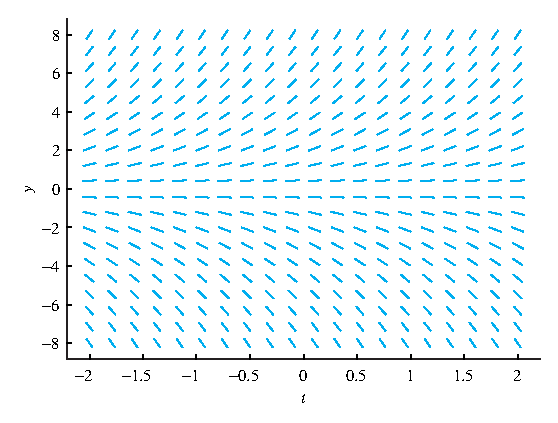
\includegraphics{Fig2.1.4.eps}
\caption{The direction field  for $y' = y$.}
\label{f2.5}
\end{figure}
\end{verbatim}
will produce Figure~\ref{f2.5}, together with its caption and a
label by which it can easily be referenced.
\begin{figure}[h!]
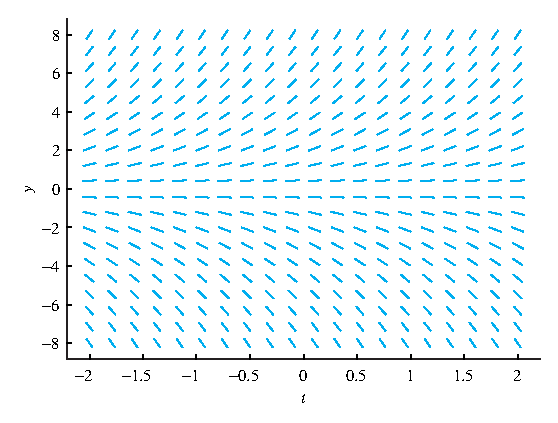
\includegraphics{Fig2.1.4.eps}
\caption{The direction field  for $y' = y$.}
\label{f2.5}
\end{figure}
(OK, I'm breaking the rules.  This one is in color. I didn't want to
waste time looking for a grayscale figure.)

You can find more information about inserting graphics into \TeX\
documents in \cite{guide}, p.157 (Section 8.1.3).

\lecture{Resources}

This is a list of resources to help you to get started if you are new to
\TeX,  \LaTeX, or  \AmS-\LaTeX, or to find  a reference
to some advanced topic if you are experienced.

\section{Books}

If you are a beginner, the AMS suggests \cite{gratz}, \emph{Math into
  \LaTeX}, by 
George Gr\"atzer 
(http://www.ams.org/bookstore-getitem/item=MLTEX.R).  This book is
published by Birkh\"auser.

A standard reference, useful for both beginners and as a reference for
more experienced authors is \cite{guide}, \emph{A Guide to \LaTeX,} by
Helmut Kopka and Patrick Daly 
(http://www.ams.org/bookstore-getitem/item=GLTEX).  Now in
its fourth edition,  published by Addison-Wesley, this book includes a
discussion of \AmS-\LaTeX.

\section{AMS web documents}

The AMS offers a wide variety of web documents offering assistance to
authors.  
\begin{list}
  {$\bullet$}
  {\leftmargin 20pt}
\item The Author Resource Center\\ (http://www.ams.org/authors/)\\  This
  is the main page. It has links to all of those that follow, and more.
\item The AMS \TeX\ Resources Home Page\\ 
  (http://www.ams.org/tex/) \\
  A link to information about \TeX\ installation and a source for the
  \AmS-\LaTeX\ collection of files.
\item Creating graphics for use in AMS books and journals (\cite{amsgraphics})\\
  (ftp://ftp.ams.org/pub/author-info/documentation/creating-graphics.pdf)\\
  This pdf document describes in detail the requirements for graphics in
  AMS publications.  We include this document in our PCMI style
  package (see Section~ \ref{package}). 
\item Frequently Asked Questions for AMS Authors\\
  (http://www.ams.org/authors/author-faq.html)\\
  An invaluable source of information about almost
  anything involving \TeX\ and AMS authorship.  You can find
  information about setting up \TeX\ on your own computer, how to put
  two figures side by side in your document, and much more.
\item User's Guide to the \texttt{amsmath} package (\cite{amsmath})\\
  (ftp://ftp.ams.org/pub/tex/doc/amsmath/amsldoc.pdf)\\
  Provides excellent guidance on the use of math in \AmS-\LaTeX.
\item Using the \texttt{amsthm} Package (\cite{amsthm})\\
(http://www.ams.org/tex/amslatex.html)\\ or directly at 
ftp://ftp.ams.org/pub/tex/doc/amscls/amsthdoc.pdf\\
This is the  definitive source for the use of the \verb-\theoremstyle-
and \verb-\newtheorem- commands discussed briefly in
Section~\ref{theorems}.  While \verb-\newtheorem- is part of standard
\LaTeXe, its use is expanded in \AmS-\LaTeX.  This expansion includes
the \verb-\theoremstyle- command as well as new numbering alternatives
and a \verb-proof- environment. 
\end{list}

\section{The PCMI style package}\label{package}
In addition, we provide a number of files.
The document style file \pcms\ is essential.  You might find the
others useful.
\begin{itemize}
\item \pcms\  --- The style file for the preparation of PCMI lecture
  series. 
\item \emph{Preparation of PCMI~Lecture~Notes} --- This document, with the
  document name \texttt{pcmistyle.pdf}.
\item \texttt{pcmistyle.tex}  --- The \TeX\ source for this document
  is an example of the use of the document class \pcms.
\item Creating graphics for use in AMS books and journals (\cite{amsgraphics})\\
  The requirements for graphics in AMS publications.
\item \texttt{pcms-l-lecture.template} --- A template for lecture
  series using the lectures option.  Change the name as appropriate to
  something ending in .tex and add what you want.
\item \texttt{pcms-l-article.template} --- A template for lecture
  series using the article option.
\end{itemize}





\begin{thebibliography}{AM}

\bibitem[AG]{amsgraphics}
\emph{Creating graphics for use in AMS books and journals,}
American Mathematical Society,  available online at \\
ftp://ftp.ams.org/pub/author-info/documentation/creating-graphics.pdf

\bibitem[AM]{amsmath}
\emph{User's Guide to the \texttt{amsmath} package}
American Mathematical Society,  available online at 
ftp://ftp.ams.org/pub/tex/doc/amsmath/amsldoc.pdf

\bibitem[AT]{amsthm}
\emph{Using the \texttt{amsthm} Package}, 
American Mathematical Society,  available online at \\
ftp://ftp.ams.org/pub/tex/doc/amscls/amsthdoc.pdf

\bibitem[GR]{gratz}
George Gr\"atzer,
\emph{Math into \LaTeX}, 3rd ed., 
Birkh\"auser, Boston (2000)

\bibitem[HK]{guide}
H. Kopka \& P. W. Daly,
\emph{A Guide to \LaTeX, Fourth edition},
Addison-Wesley Professional, New York, NY (November 2003)

\end{thebibliography}


\end{document}